\chapter{\label{appendix:spinvalve}Tb--Dy Molecular Spin Valve}

\minitoc

\section{Introduction}\label{sec:spinvalve:introduction}

Typically a spin valve is a trilayered device in which a paramagnetic material (also called \textit{spacer}) of interest is sandwiched between two ferromagnetic (FM) electrodes of different coercitivities, so they may be independetly controlled by just one magnetic field.

One of the FM acts as a \textit{spin injector}, meaning that, if an electrical bias is applied, spins from a population $P_0$ are injected from the quasi-Fermi level into the paramagnet. The second paramagnet is called \textit{spin detector} and owns its name to the fact that it provides unequal spin-up and
spin-down DOS at the Fermi level, thus preferentially transmitting spins of one particular orientation.
Overall this would result in a low device resistance when the magnetization of the two magnets are parallel but when their alignement is antiparallel the resistance would be high\footnote[1]{This argument is strictly valid in case the distance between the two magnets is smaller than the spin-diffusion length $\lambda_s\sim \log{(\frac{P}{P_0})}^{-1}$, and P depends of the spacer length.}.

A couple of years back it has been envisioned to mimick the same device but entirely with a supramolecular structure. One of the first proposal discussed the possibility to control preferentially spin currents when these where injected through porphyrins adsorbed on a single CNT~\cite{urdampilleta2011supramolecular}.

\begin{figure}[hbtp]
    \begin{center}
        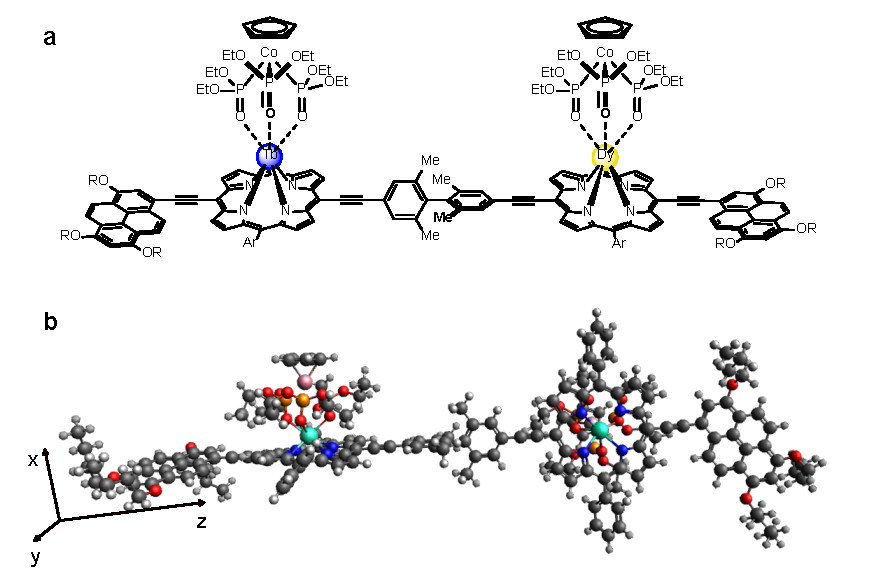
\includegraphics[width=\textwidth]{text/spinvalve_mol_tb_opt.pdf}
        \caption[Tb--Dy Spin Valve: Molecular Structure and Tight-Binding-Optimised Geometry]
        {\textbf{a,} Molecular structure of the Tb--Dy porphyrin. In blue and white are highlighted the rare-earth metal centres. R = --\ce{C12H25}; Ar = 3,5-bis(trihexylsilyl)phenyl.
            \textbf{b,} Tight-binding optimised geometry. The --R groups have been discarded to simplify the geometry, and since they do not impact any electronic or magnetic properties. The total number of atoms for this structure is $N=405$ atoms. Reference system referes to the orientations of the 3D vector magnet in the dilution refrigerator.}
        \label{fig:spinvalve_structure_geom_optimised}
    \end{center}
\end{figure}

The aim of the project is to observe magnetoresistance for a double-porphyrin supramolecular comples, thus demonstrating spin valve capabilities. This requires, first, to establish if the device conductance is suppressed for at certain field value. Since it was not possible to study the individual building blocks of the double porphyrin,  we atttempted to study the entire molecule.

\section{Experimental and Computational Methods}\label{sec:spinvalve:methods}

Before attempting any transport experiments we carried out an explorative \textit{in-silico} analysis to characterise the magnetic properties of the double porphyrin. To this end, a first important step was to define the type of functional to use. In this respect, \gls{LDA} and \gls{GGA} functionals are concave and locals/semi-locals, meaning that the charge density is calculated locally, and so they notoriously tend to describe the electron density for locally respected to the true (unknown) functional. This often leads to an underestimate of the ionization potential and to an overestimate of the electron affinity. This weakness of local functionals is of paramount importance to address especially in strongly-correlated system such as this one, where the presence of $f-$electrons in a delocalised matrix imposes to heavily correct the systematic error generated by local functionals otherwise resulting in inversions when the spinorbitals are filled.

One strategy to overcome this is to use hybrid functionals, which have been introduced since the early 90s and they include, through various scheme, an exact contribution (Hartree--Fock) to a DFT functional~\cite{stephens1994ab, becke1993new}. This procedure, however, is notoriously computationally heavy and one must proceed with caution to even run some preliminary tests. Indeed, because the HF involves the computational of four-body integrals, one has to perform $N(N-1)$ operations to evaluate these integrals. This translates in a computational time complexity of $\mathcal{O}_\textrm{DFT}*\mathcal{O}_\textrm{HF}=N^5$. When the overlap between the bielectronic integrals is small, algorithmic optimizations typically bring the computational complexity time down to $\mathcal{O}(N^{3-3.5})$. Therefore, if the time employed to run a calculation of about $N=40$ is about 2 days, if then the system size is increased to $N=400$ the calculation time would be $(400/40)^3=1000$ longer, roughly corresponding to 5 years and half. This assuming the best case scenario in which the calculation scales as a power of three.

Preliminary results have been obtained by adopting the PBEh functional which introduce a 42 percent of exact (HF) exchange and implement a series of correcctions which has previously led to reasonable results even in case of big systems ($N\simeq150$ atoms)~\cite{rohrdanz2009long, atalla2013hybrid}.

Fig.~\ref{fig:spinvalve_structure_DFT_optimised} shows the structure of the double porphyrin optimised at DFT level. The molecule was first reduced in dimension by removing the majority of the anchoring group attached at the two terminal position. The total number of atoms was reduced fom 405 to 298, which still represents an important system to simulate \textit{ab-initio}. In order the keep the initial test time short, we choose a aug-cc-pVDZ-DK basis set.

\section{Results}

\subsection{Computational}\label{sec:spinvalve:computational}
All measurements were carried out at cryogenic temperatures. The sample was dissolved in toluene and presented eccellent solubility even without shaking. The solution was kept in the fridge for almost an year and MALDI performed at intervals of $\sim$4 months confirmed the structure stability even when kept in solution in the fridge. Solution of $\sim$\SI{8}{\micro\litre} were dropcasted on top of graphene tunnel junctions as already outline in the preceeding chapters, and transport properties performed in the Oxford Triton 200 Dilution Refrigerator.

Since the energy differences involved between the FM and the AFM configuration are presumably small, one has to first heavily optimise the geometry so there is a very small error on the bonding forces. Unfortunately a crystal structure of this molecule was not available at the time when this project was carried out. A strong polar implicit solvent (acetonitrile, \ce{MeCN}) was employed in order to avoid any buckling up of the supramolecular structure.

The problem with this system is twofold: on the one hand you want to go and see presumably small energy differences due to the spins of the different pieces of the molecules first the geometry has to be optimised in a pushy way, so there has to be a very small error on the bonding forces. After that you have to do the FM count first, then flip the magnetisation f orbitals to one side and see the energy difference with the AFM structure. And you want to see this both when the anchor molecules are flat and when they are tilted. So in total one account with four cases.

The challenge with this system is twofold: on the one hand, energy differences due to the spins of the different sections of the molecules will be very small, and on the other hand, the geometry must be optimised so there is minimal inaccuracy in the bonding forces. Then, an FM estimation must be performed before flipping the magnetisation of the $f-$orbitals and comparing the energy difference with the AFM structure. There are a total of four scenarios to examine, as calculations must be conducted both when the anchor molecules are flat and when they are inclined.

The three rare-earth--oxygen bonds provided by the tripodal (Kl{\"a}ui) ligand are not collinear with the nitrogens belonging to the porphyrinic ring and so they force the porphyrin ring to undergo into a structural distortion.

The structure seems to indicate it preferentially orientates the two aryl rings in the middle perpendicolar to each other. One should then take the full-optimised geometry, carefully rotate along the middle triple bond and then explore the four different configurations outline above.

%This result was carried out by employing a 128 GB-big node  machine with 8 runs of 48h long each.

\begin{figure}[hbtp]
    \begin{center}
        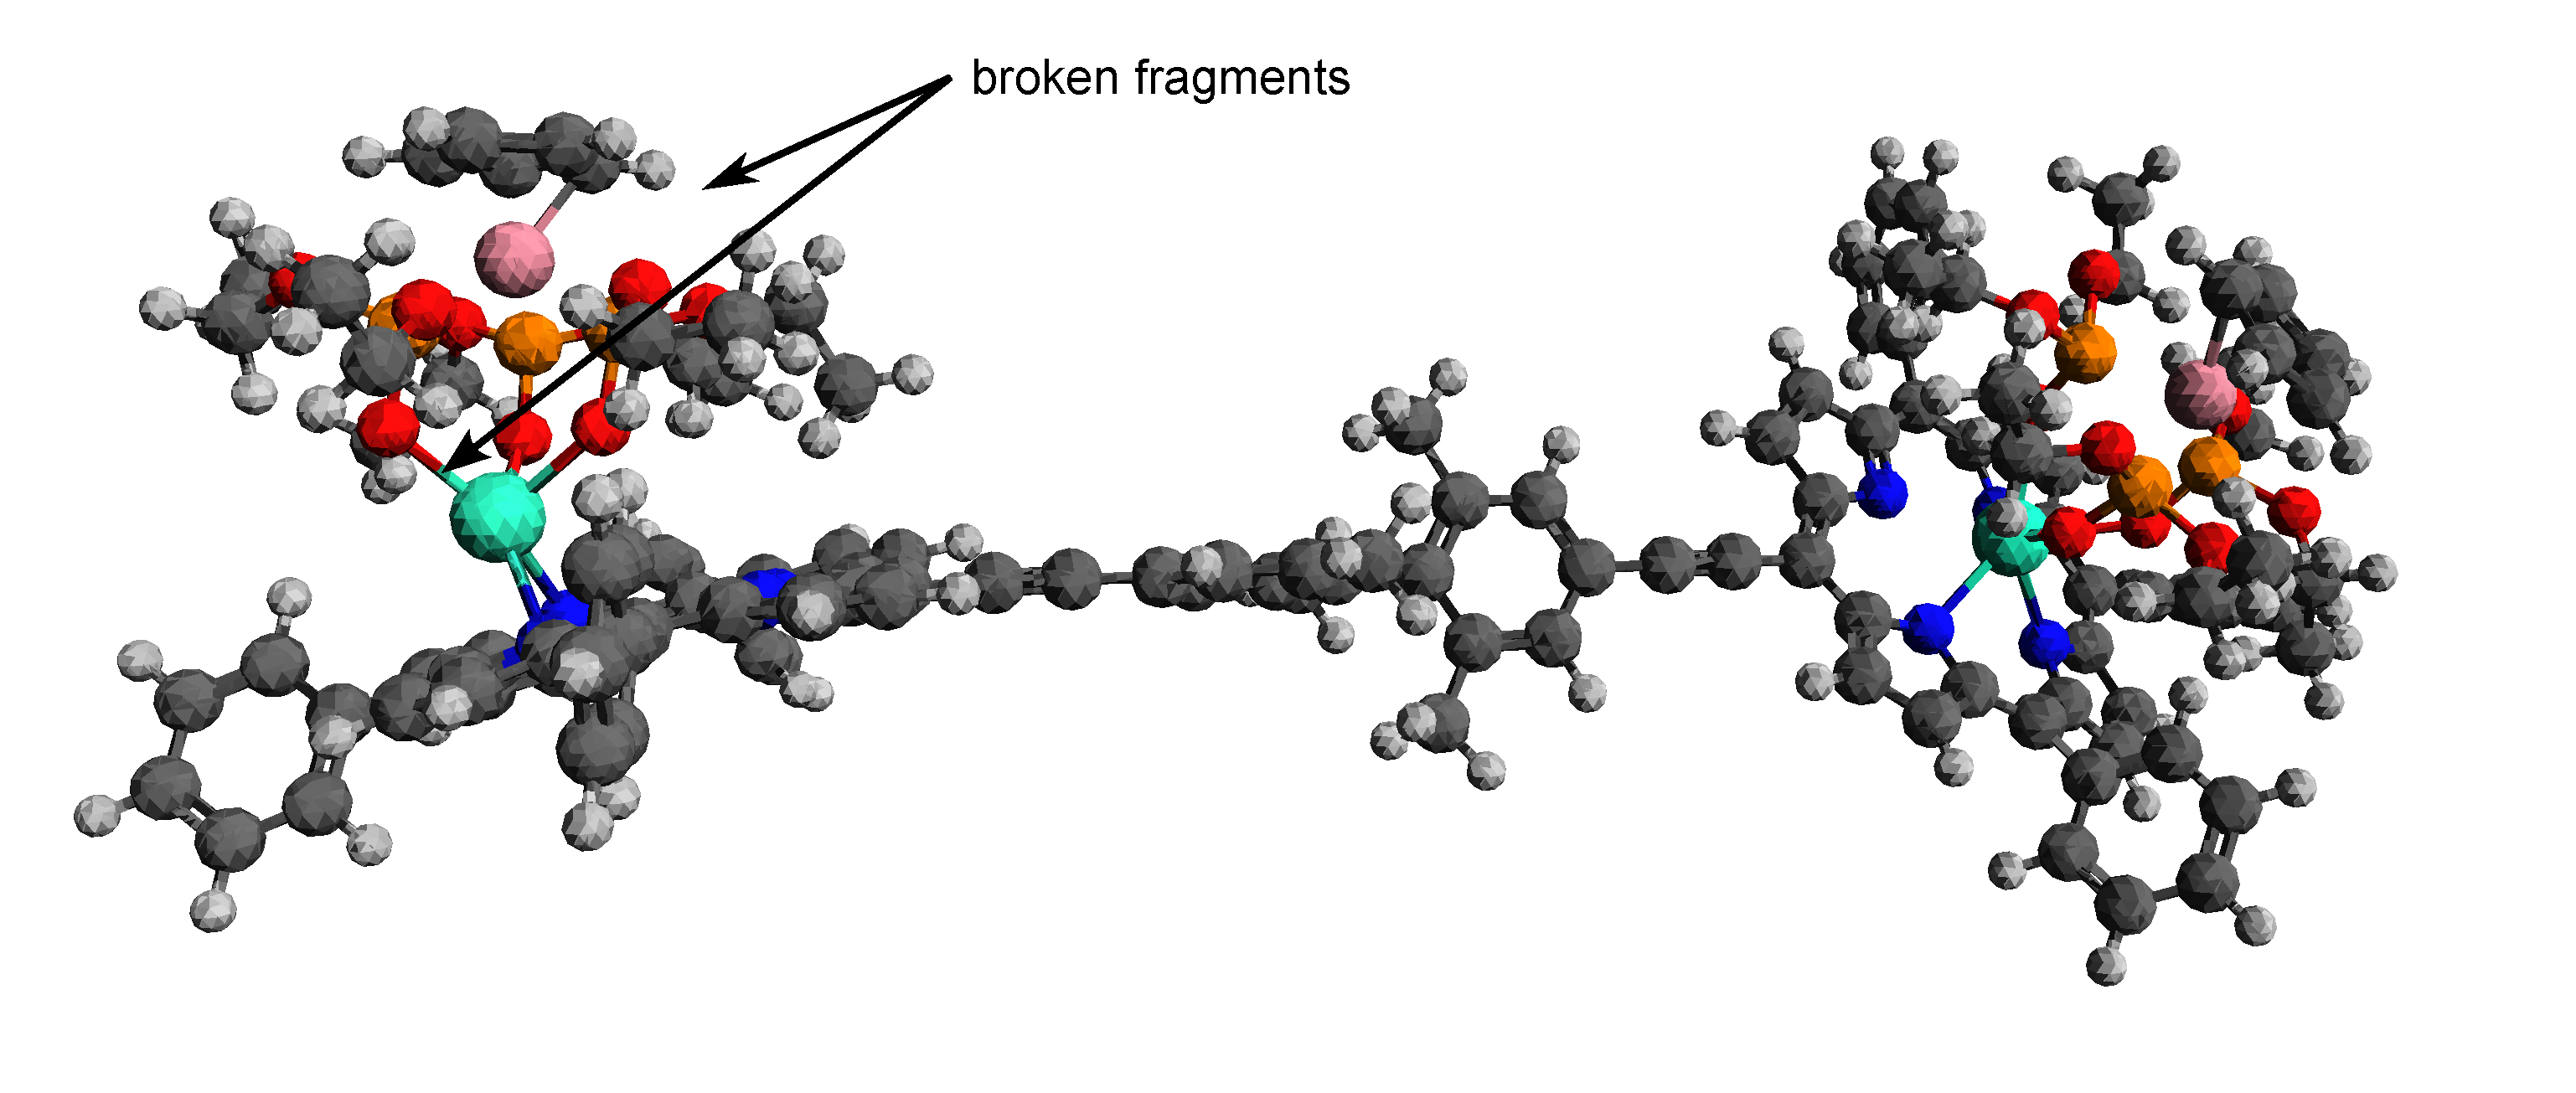
\includegraphics[width=\textwidth]{text/dft_geom_broken.pdf}
        \caption[Tb--Dy Spin Valve: DFT-Optimised Geometry]
        {Tb--Dy structure when optimsed at the DFT level. Simulation protocol is detailed in the main text. While the DyP seems to remain intact, the TbP present several critical breaking points in the structure.}
        \label{fig:spinvalve_structure_DFT_optimised}
    \end{center}
\end{figure}


After 8 runs of 48h each the structure have started to break down, when the accuracy on the forces was one order of magnitude higher ($\sim$\SI{1e-4}{\atomicmassunit}) than the one is required to satisfactorily exit the scf cycle. since the system has many degrees of freedom the scaling is not linear to when you get to that limit so reaching the required level on the force might have taken longer than than the time the reached this accuracy level.

The calculation was interrupted as the structure started to break down. Fig.~\ref{fig:spinvalve_structure_DFT_optimised} shows the geometry at the last scf cycle. Breaking of the structure during the geometry optimisation step is often a clear indication that the filling of the spinorbitals is not correct and a detailed study of the two separate porphyrin units is required.


\begin{figure}[hbtp]
    \begin{center}
        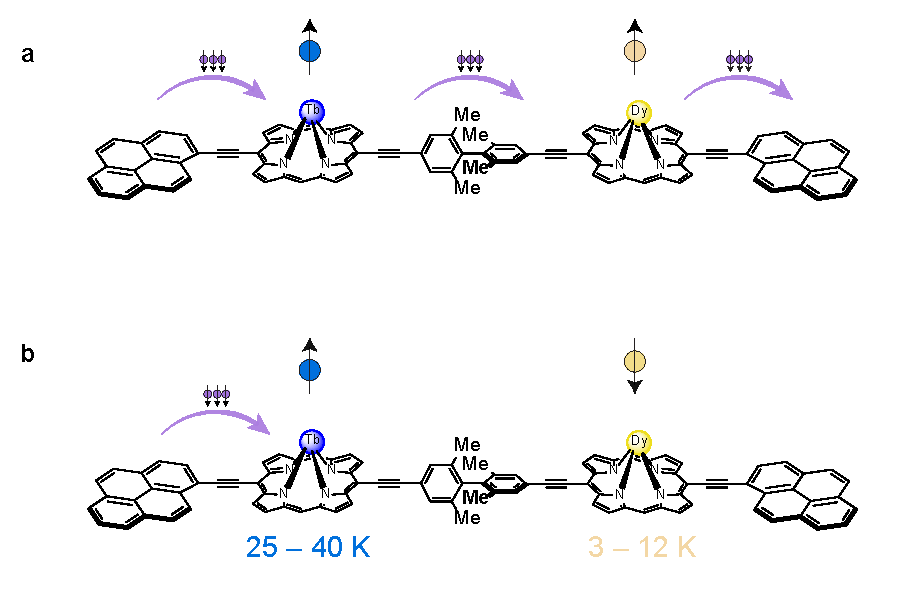
\includegraphics[width=\textwidth]{text/spinvalve_functioning.pdf}
        \caption[Tb--Dy Spin valve: Functioning Mechanism]
        {\textbf{a,} When $B=0$, the Pauli exclusion principles guarantees that a spin-down polarised current may travel across the whole structure resulting in overall low resistance (high $G$). \textbf{b,} When $B\neq0$, paired spins act as spin blockade and no spin-polarised current can flow across both metals due to the Pauli principle. Indicated are the respective energy splitting amongst the magnetic level for each rare-earth when a magnetic field lifts the degeneracy between spin-up and spin-down states.}
        \label{fig:spinvalve_mechanism}
    \end{center}
\end{figure}

\subsection{Coulomb-Blockade Spectroscopy}

We report here the transport measurements we have acquired for the Dy--Tb double porphyrin. Albeit we intensly ($\sim 6$ months) searched for reproducible features, we did not manage to complete the full set of measurements planned due to (1) irreproducible features and (2) jumping during gate and bias scans, especially when a magnetic field was applied, and possibly due to charge trapped into the \ce{HfOx} substrate.

Although it is not clear at this stage why these devices lacked in reproducibility, one possibility could be due to the overall conformation of the structure. \Gls{TB}-level optimisation suggests that the two biphenyl units prefer to stay rotate \SI{90}{\degree} each other, causing the complete rotation of the TbP part. Although anchoring groups were omitted in our optimisation, we bieleve that this effect might result in worsen $\pi$--$\pi$ interactions established between the anchoring groups and the graphene leads. Different linking groups between the two porphyrin units could then lead to improved reproducibilities.

\begin{figure}[hbtp]
    \begin{center}
        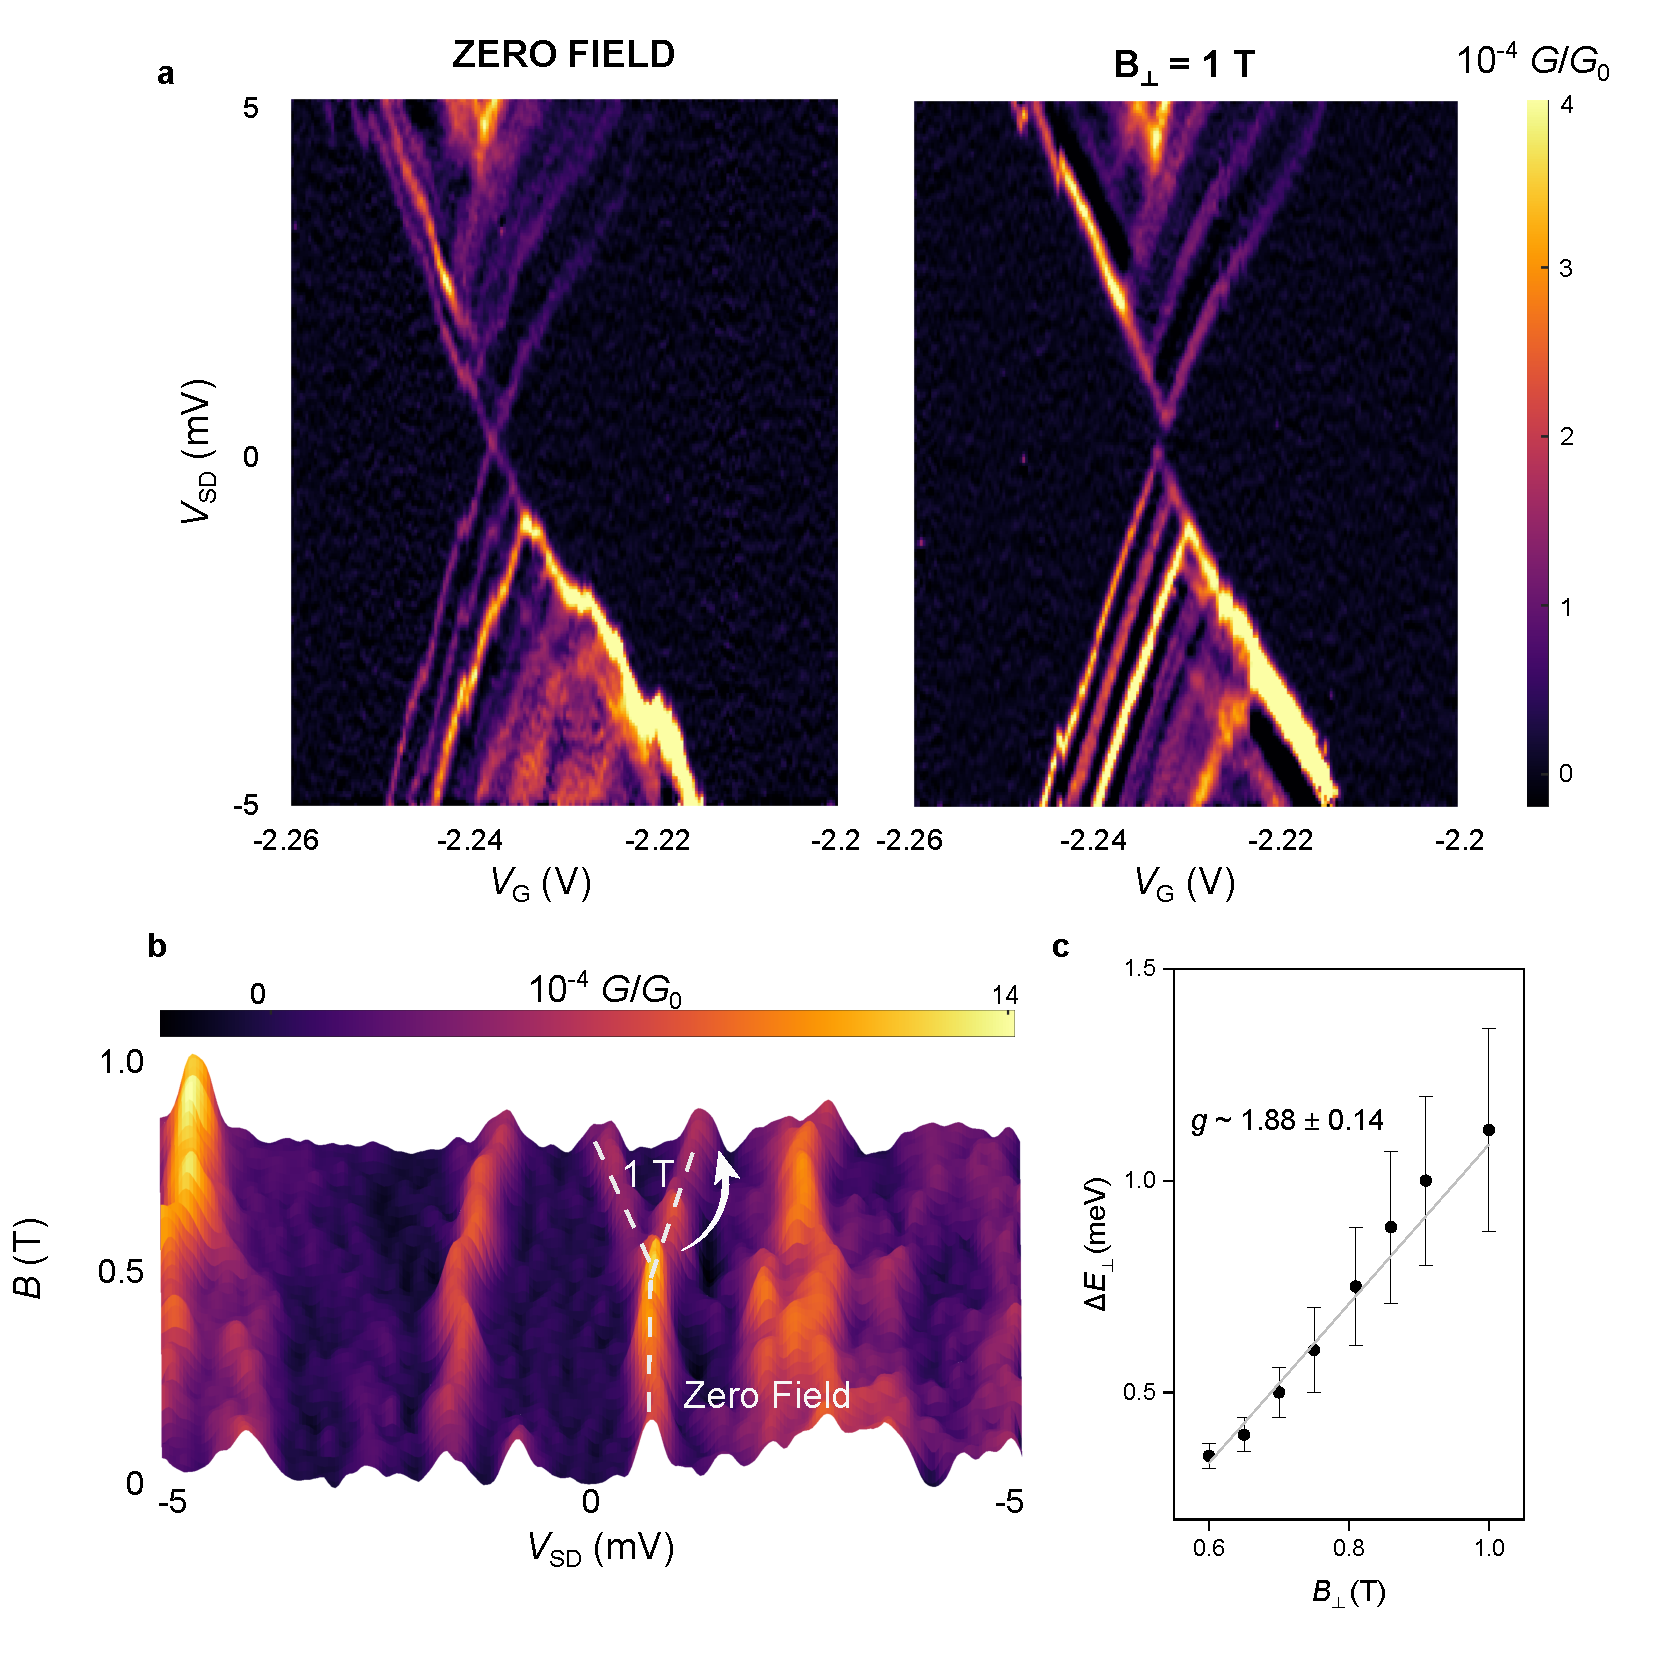
\includegraphics[width=\textwidth]{text/-2.23V_diamond.pdf}
        \caption[Tb--Dy Spin Valve: Field-Sweep Analysis of the Coulomb Diamond at \SI{-2.23}{\volt}]
        {
            \textbf{a}, Zero-field stability diagram. Excited states inside the diamond are visible, as well as negative differential conductance at positive bias.
            \textbf{b}, The same diamond when $\SI{1}{\tesla}$ is applied transversal to the porphyrin plane. Differential conductance are still present at postive bias, and we also observe an in increase in the conductance of the left diamond-edge (brighter line). Although it might be possible to observe Pauli Spin blockade.
            \textbf{c}, Magnetic-field evolution of the bias curves in the same gate voltage range as (a). The peak close to zero bias split $B_\perp\gtrapprox\SI{0.5}{\tesla}$
            \textbf{d}, By assuming the splitting is cause by the Zeeman splitting we estimate a $g$ factor of $\simeq\si[separate-uncertainty = true]{1.88(0.14)}$
        }
        \label{fig:--2.23V_diamond}
    \end{center}
\end{figure}
\newpage
\begin{figure}[hbtp]
    \begin{center}
        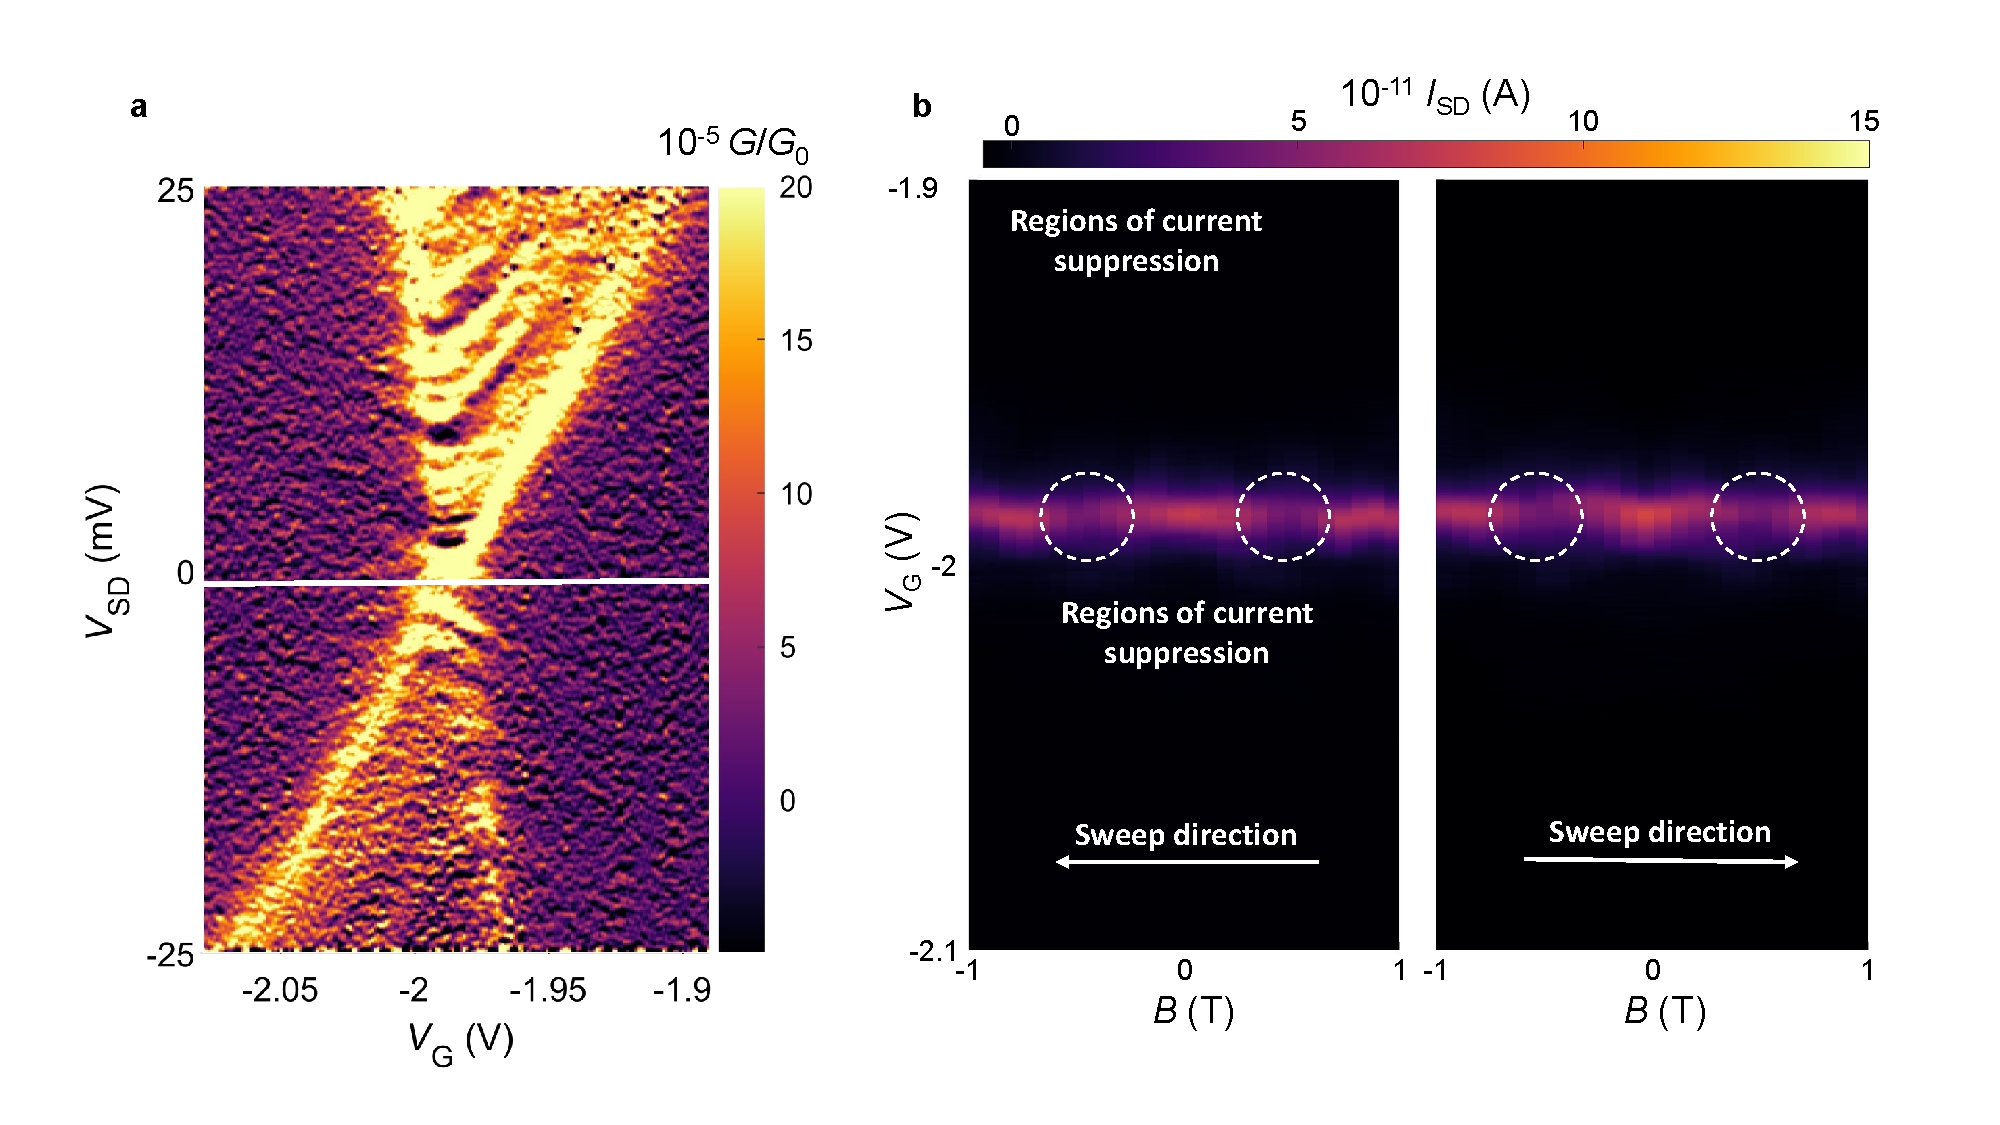
\includegraphics[width=\textwidth]{text/-2V_diamond_field_sweep.pdf}
        \caption[Tb--Dy Spin Valve: Field-Sweep Analysis of the Coulomb Diamond at \SI{-2}{\volt}]
        {
            \textbf{a,} Diamond for a different device at \SI{-2}{\volt}
            \textbf{b,} We measured the current at very low bias ($V_\textrm{SD}=\SI{1}{\milli\volt}$) as a function of the perpendicualar field $B_\perp$ and observed reproducible regions of current suppressed when the field was swept both in forward an backward direction.
        }
        \label{fig:-2V_diamond_field_sweep}
    \end{center}
\end{figure}
\newpage
\begin{figure}[hbtp]
    \begin{center}
        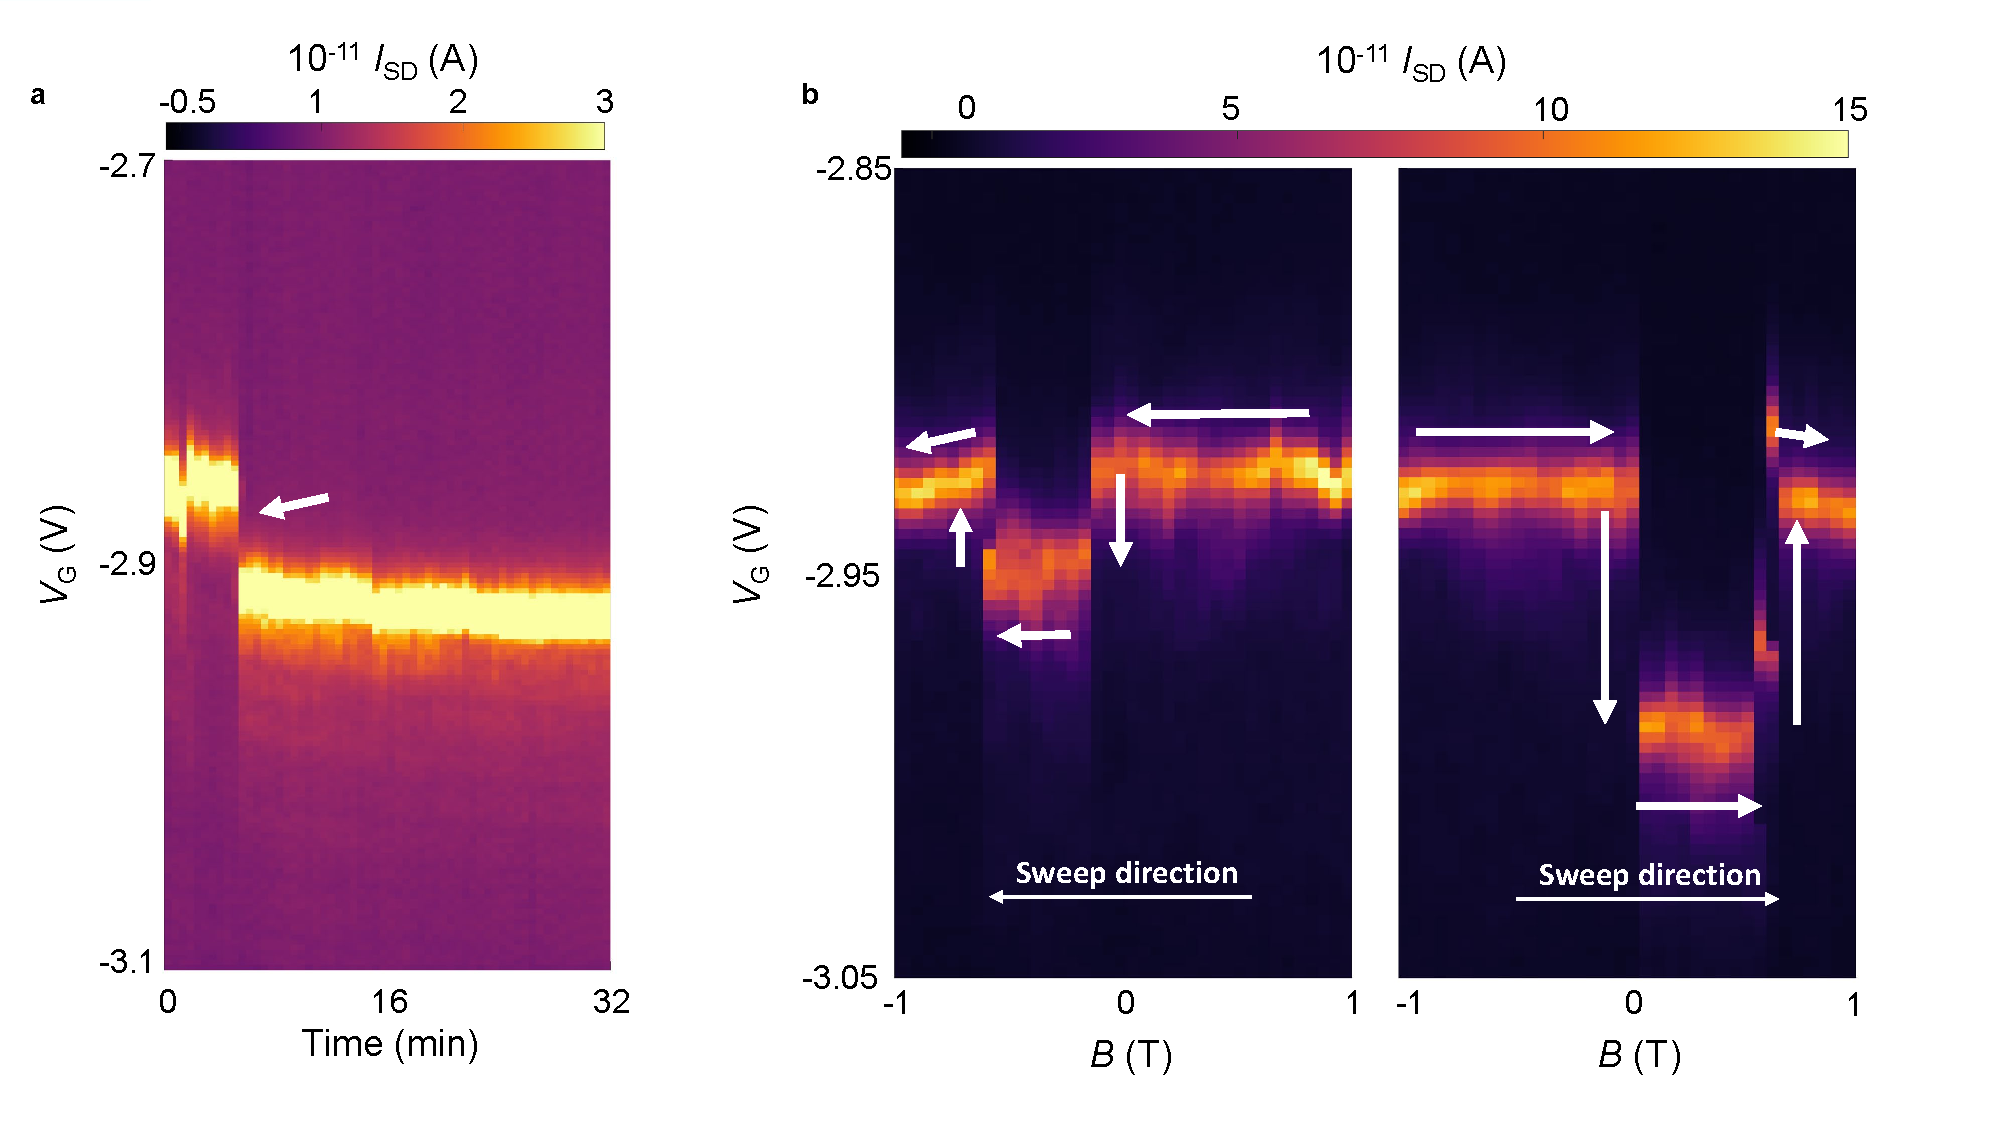
\includegraphics[width=\textwidth]{text/-3V_diamond_field_sweep.pdf}
        \caption[Tb--Dy Spin Valve: Field-Sweep Analysis of the Coulomb Diamond at \SI{-3}{\volt}]
        {
            \textbf{a,} Time trace of the current at fixed bias ($V_\textrm{SD}=\SI{3}{\milli\volt}$). Arrow indicate the occurance of a charge jump during the acquisition which prevent further investigations.
            \textbf{b,} Current evolution as a function of the transversal field and the gate demonstrating non-reproducible charge jumps when the field sweep was inverted.
        }
        \label{fig:-3V_diamond_field_sweep}
    \end{center}
\end{figure}

\section{Concluding Remarks}

In this chapter we briefly commented the results obtained with \gls{DFT} and electron transport on a Tb--Dy double porphyrin.
Due to time limitations we were not able to finish the project, and therefore we cannot present a conclusive outlook. However, we discuss here current problems and future steps.

The key difficulty from a computational standpoint is the unknown crystal structure, which forced us to start with an unoptimised-input geometry that broke during the self-consistent-field cycles. The lack of reproducible-experimental results may be explained by considering that the preferential orientation of the anchoring group in the ground state appears to have the two linking aryl groups perpendicular to each other, resulting in one porhyrin unit completely tilted and preventing a good anchoring with the graphene leads.

While we are still unable to interpret the spectra and to determine whether or not this molecule display a spin-valve behaviour, one device displayed peak splitting when the field was swept up to \SI{1}{\tesla} along the direction perpendicular to the molecule extension plane.  Intuitively, this might be explained by the Zeeman interaction $\mathcal{H}_Z = -\vec{\mu}\cdot\vec{B}$ which couples the Dy magnetic moment with magnetic field. No zero-field splitting of these states are observed which might hint the absence of exchange interactions~\cite{pei2022exchange}. Additional information about the energy difference between the FM and the AFM configurations might be obtained by modelling the problem with an Hubbard model as recently performed for simular porphyrin systems~\cite{thomas2021charge}.


\section{Project Overview}

The Tb--Dy double porphyrin discussed in this project was designed and synthesised by Dr Keith Andrews and prof.\ Harry Anderson. I thanked each of them, as well as Dr Alex Gee, for the several devices we measured together and independetly.

